\documentclass[
11pt, % Set the default font size, options include: 8pt, 9pt, 10pt, 11pt, 12pt, 14pt, 17pt, 20pt
%t, % Uncomment to vertically align all slide content to the top of the slide, rather than the default centered
%aspectratio=169, % Uncomment to set the aspect ratio to a 16:9 ratio which matches the aspect ratio of 1080p and 4K screens and projectors
]{beamer}

\graphicspath{{images/}{./}} % Specifies where to look for included images (trailing slash required)

\usepackage{watermark}
\usepackage{graphicx}  % Para incluir imágenes si deseas usar una imagen como marca de agua
\usepackage{array}
\usepackage[utf8]{inputenc}
\usepackage[spanish]{babel}
\usepackage{circuitikz} % Paquete para diagramas de circuitos eléctricos
\usepackage{tikz}
\usetikzlibrary{shapes.geometric, arrows.meta, positioning}
\usepackage{smartdiagram}
\usepackage{eso-pic}
\usepackage{lmodern}
\usepackage{xcolor}
\usepackage{booktabs}
\usepackage{url}

\definecolor{universityblue}{RGB}{0, 102, 204}
\definecolor{universitygreen}{RGB}{0, 153, 0}
\definecolor{universityyellow}{RGB}{255, 215, 0}

\setbeamercolor{structure}{fg=universityblue}
\setbeamercolor{alerted text}{fg=universitygreen}
\setbeamercolor{background canvas}{bg=white}


% Agregar logo
\logo{
\includegraphics[width=1cm]{logo.jpeg}} % Cambia "logo.png" por la ruta de tu imagen

\usepackage{booktabs} % Allows the use of \toprule, \midrule and \bottomrule for better rules in tables

%----------------------------------------------------------------------------------------
%	SELECT LAYOUT THEME
%----------------------------------------------------------------------------------------

% Beamer comes with a number of default layout themes which change the colors and layouts of slides. Below is a list of all themes available, uncomment each in turn to see what they look like.

%\usetheme{default}
%\usetheme{AnnArbor}
%\usetheme{Antibes}
%\usetheme{Bergen}
%\usetheme{Berkeley}
%\usetheme{Berlin}
%\usetheme{Boadilla}
\usetheme{CambridgeUS}
%\usetheme{Copenhagen}
%\usetheme{Darmstadt}
%\usetheme{Dresden}
%\usetheme{Frankfurt}
%\usetheme{Goettingen}
%\usetheme{Hannover}
%\usetheme{Ilmenau}
%\usetheme{JuanLesPins}
%\usetheme{Luebeck}
%\usetheme{Madrid}
%\usetheme{Malmoe}
%\usetheme{Marburg}
%\usetheme{Montpellier}
%\usetheme{PaloAlto}
%\usetheme{Pittsburgh}
%\usetheme{Rochester}
%\usetheme{Singapore}
%\usetheme{Szeged}
%\usetheme{Warsaw}

%----------------------------------------------------------------------------------------
%	SELECT COLOR THEME
%----------------------------------------------------------------------------------------

% Beamer comes with a number of color themes that can be applied to any layout theme to change its colors. Uncomment each of these in turn to see how they change the colors of your selected layout theme.

%\usecolortheme{albatross}
%\usecolortheme{beaver}
%\usecolortheme{beetle}
%\usecolortheme{crane}
%\usecolortheme{dolphin}
%\usecolortheme{dove}
%\usecolortheme{fly}
%\usecolortheme{lily}
%\usecolortheme{monarca}
%\usecolortheme{seagull}
%\usecolortheme{seahorse}
%\usecolortheme{spruce}
%\usecolortheme{whale}
%\usecolortheme{wolverine}

%----------------------------------------------------------------------------------------
%	SELECT FONT THEME & FONTS
%----------------------------------------------------------------------------------------

% Beamer comes with several font themes to easily change the fonts used in various parts of the presentation. Review the comments beside each one to decide if you would like to use it. Note that additional options can be specified for several of these font themes, consult the beamer documentation for more information.

\usefonttheme{default} % Typeset using the default sans serif font
%\usefonttheme{serif} % Typeset using the default serif font (make sure a sans font isn't being set as the default font if you use this option!)
%\usefonttheme{structurebold} % Typeset important structure text (titles, headlines, footlines, sidebar, etc) in bold
%\usefonttheme{structureitalicserif} % Typeset important structure text (titles, headlines, footlines, sidebar, etc) in italic serif
%\usefonttheme{structuresmallcapsserif} % Typeset important structure text (titles, headlines, footlines, sidebar, etc) in small caps serif

%------------------------------------------------

%\usepackage{mathptmx} % Use the Times font for serif text
\usepackage{palatino} % Use the Palatino font for serif text

%\usepackage{helvet} % Use the Helvetica font for sans serif text
\usepackage[default]{opensans} % Use the Open Sans font for sans serif text
%\usepackage[default]{FiraSans} % Use the Fira Sans font for sans serif text
%\usepackage[default]{lato} % Use the Lato font for sans serif text

%----------------------------------------------------------------------------------------
%	SELECT INNER THEME
%----------------------------------------------------------------------------------------

% Inner themes change the styling of internal slide elements, for example: bullet points, blocks, bibliography entries, title pages, theorems, etc. Uncomment each theme in turn to see what changes it makes to your presentation.

%\useinnertheme{default}
\useinnertheme{circles}
%\useinnertheme{rectangles}
%\useinnertheme{rounded}
%\useinnertheme{inmargin}

%----------------------------------------------------------------------------------------
%	SELECT OUTER THEME
%----------------------------------------------------------------------------------------

% Outer themes change the overall layout of slides, such as: header and footer lines, sidebars and slide titles. Uncomment each theme in turn to see what changes it makes to your presentation.

%\useoutertheme{default}
%\useoutertheme{infolines}
%\useoutertheme{miniframes}
%\useoutertheme{smoothbars}
%\useoutertheme{sidebar}
%\useoutertheme{split}
%\useoutertheme{shadow}
%\useoutertheme{tree}
%\useoutertheme{smoothtree}

%\setbeamertemplate{footline} % Uncomment this line to remove the footer line in all slides
%\setbeamertemplate{footline}[page number] % Uncomment this line to replace the footer line in all slides with a simple slide count

%\setbeamertemplate{navigation symbols}{} % Uncomment this line to remove the navigation symbols from the bottom of all slides

%----------------------------------------------------------------------------------------
%	PRESENTATION INFORMATION
%----------------------------------------------------------------------------------------

\title[Metodología de Investigación]{Metodología para el estudio universitario} % The short title in the optional parameter appears at the bottom of every slide, the full title in the main parameter is only on the title page

%\subtitle{Optional Subtitle} % Presentation subtitle, remove this command if a subtitle isn't required

\author[Edison Achalma]{Edison Achalma} % Presenter name(s), the optional parameter can contain a shortened version to appear on the bottom of every slide, while the main parameter will appear on the title slide

\institute[CAU - UNSCH]{Corporación Académica Universitaria CAU - UNSCH \\ \smallskip \textit{achalmed.18@gmail.com}} % Your institution, the optional parameter can be used for the institution shorthand and will appear on the bottom of every slide after author names, while the required parameter is used on the title slide and can include your email address or additional information on separate lines

\date[\today]{Sesión 08 \\ \today} % Presentation date or conference/meeting name, the optional parameter can contain a shortened version to appear on the bottom of every slide, while the required parameter value is output to the title slide

%----------------------------------------------------------------------------------------


\begin{document}
% Página de título
\begin{frame}
	\titlepage
\end{frame}

% Diapositiva de contenido
% Configuración: Incluir índice automáticamente en cada sección

\AtBeginSection[]{
	\begin{frame}{Índice de la Sección}
		\tableofcontents[currentsection] % Índice automático de la sección actual
	\end{frame}
}

\section{Los Tres Niveles de Internet}

\begin{frame}{La Internet Superficial / Surface Web}

	\begin{columns}
		\column{0.5\textwidth}
		\begin{itemize}
			\item Comprende páginas web indexadas por motores de búsqueda convencionales.
			\item Representa solo el 30\% de la información disponible en internet.
			\item \textbf{Ejemplos}: Google, Facebook, YouTube.
		\end{itemize}
		\column{0.5\textwidth}
		\begin{figure}[H]
			\centering
			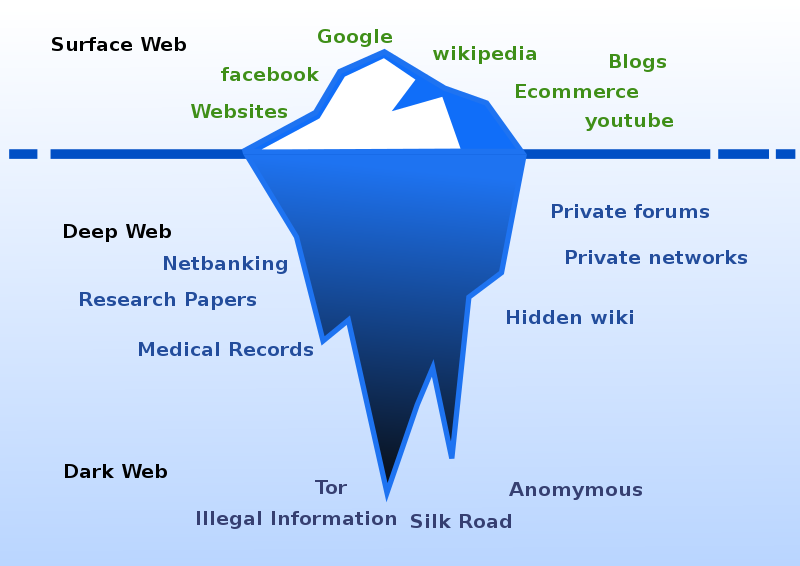
\includegraphics[width=1\linewidth]{images/image03}
		\end{figure}
	\end{columns}

\end{frame}

\begin{frame}{La Internet Profunda / Deep Web}

	\begin{columns}
		\column{0.5\textwidth}
		\begin{itemize}
			\item Contenidos dinámicos o protegidos que no son accesibles por motores de búsqueda
			      estándar.
			\item Requiere autenticación (usuario/contraseña).
			\item \textbf{Ejemplos}: Bases de datos, \textbf{Trabajos de investigación}, servicios bancarios, Dropbox, Gmail.
		\end{itemize}
		\column{0.5\textwidth}
		\begin{figure}[H]
			\centering
			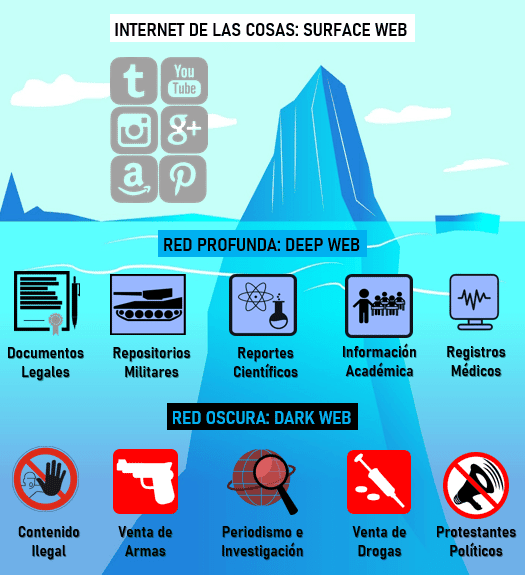
\includegraphics[width=1\linewidth]{images/image04}
		\end{figure}
	\end{columns}

\end{frame}

\begin{frame}{La Internet Oscura / Dark Web}
	\begin{itemize}
		\item Páginas ocultas sin enlaces, accesibles solo a través de redes privadas
		      virtuales.
		\item Ejemplo de acceso: Tor.
	\end{itemize}

	\begin{figure}[H]
		\centering
		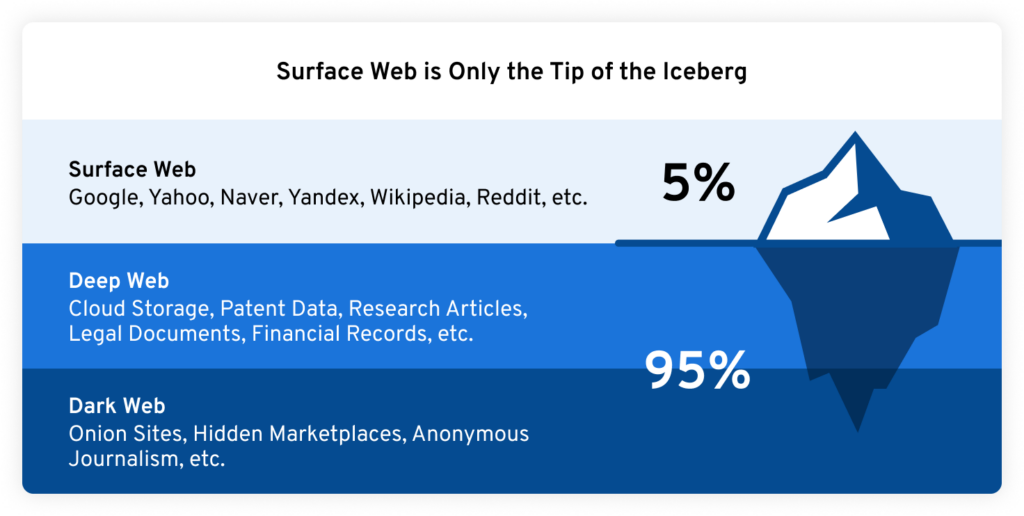
\includegraphics[width=1\linewidth]{images/image01}
	\end{figure}

\end{frame}

\section{Infoxicación}

\begin{frame}{Características de la Información en Internet}
	\begin{itemize}
		\item Cobertura global.
		\item Actualización constante.
		\item Acceso inmediato.
		\item Sobrecarga de información dificulta el análisis y selección.
		\item No toda la información es relevante, confiable o útil.
	\end{itemize}
\end{frame}

\section{Buscadores}

\begin{frame}{Buscadores}
	\begin{itemize}
		\item Sitios web que consultan bases de datos con direcciones de páginas web y su
		      contenido.
		\item Uso de palabras clave para obtener una lista de resultados.
	\end{itemize}

	\vspace{0.5cm} % Adds some vertical space before the icons

	\begin{columns}[T] % [T] aligns columns at the top
		\column{0.25\textwidth}
		\centering
		
\includegraphics[width=0.8\linewidth]{images/ecosia_icon}

		\column{0.25\textwidth}
		\centering
		
\includegraphics[width=0.4\linewidth]{images/bing_icon}

		\column{0.25\textwidth}
		\centering
		
\includegraphics[width=0.8\linewidth]{images/duckduckgo_icon}

		\column{0.25\textwidth}
		\centering
		
\includegraphics[width=0.8\linewidth]{images/wolaframalpha_icon}
	\end{columns}
\end{frame}

\begin{frame}{Planificación de la Búsqueda}
	\begin{itemize}
		\item Google domina con más del 90\% de las búsquedas.
		\item Google no busca en tiempo real, sino en su base de datos indexada.
		\item Estrategias: Búsqueda en otros idiomas, uso del traductor, guardar información para revisión posterior.
	\end{itemize}
\end{frame}

\begin{frame}{DuckDuckGo}
	\begin{itemize}
		\item Alternativa a Google que enfatiza la privacidad del usuario.
		\item No rastrea ni guarda la información de búsqueda de los usuarios.
	\end{itemize}

	\begin{figure}[H]
		\centering
		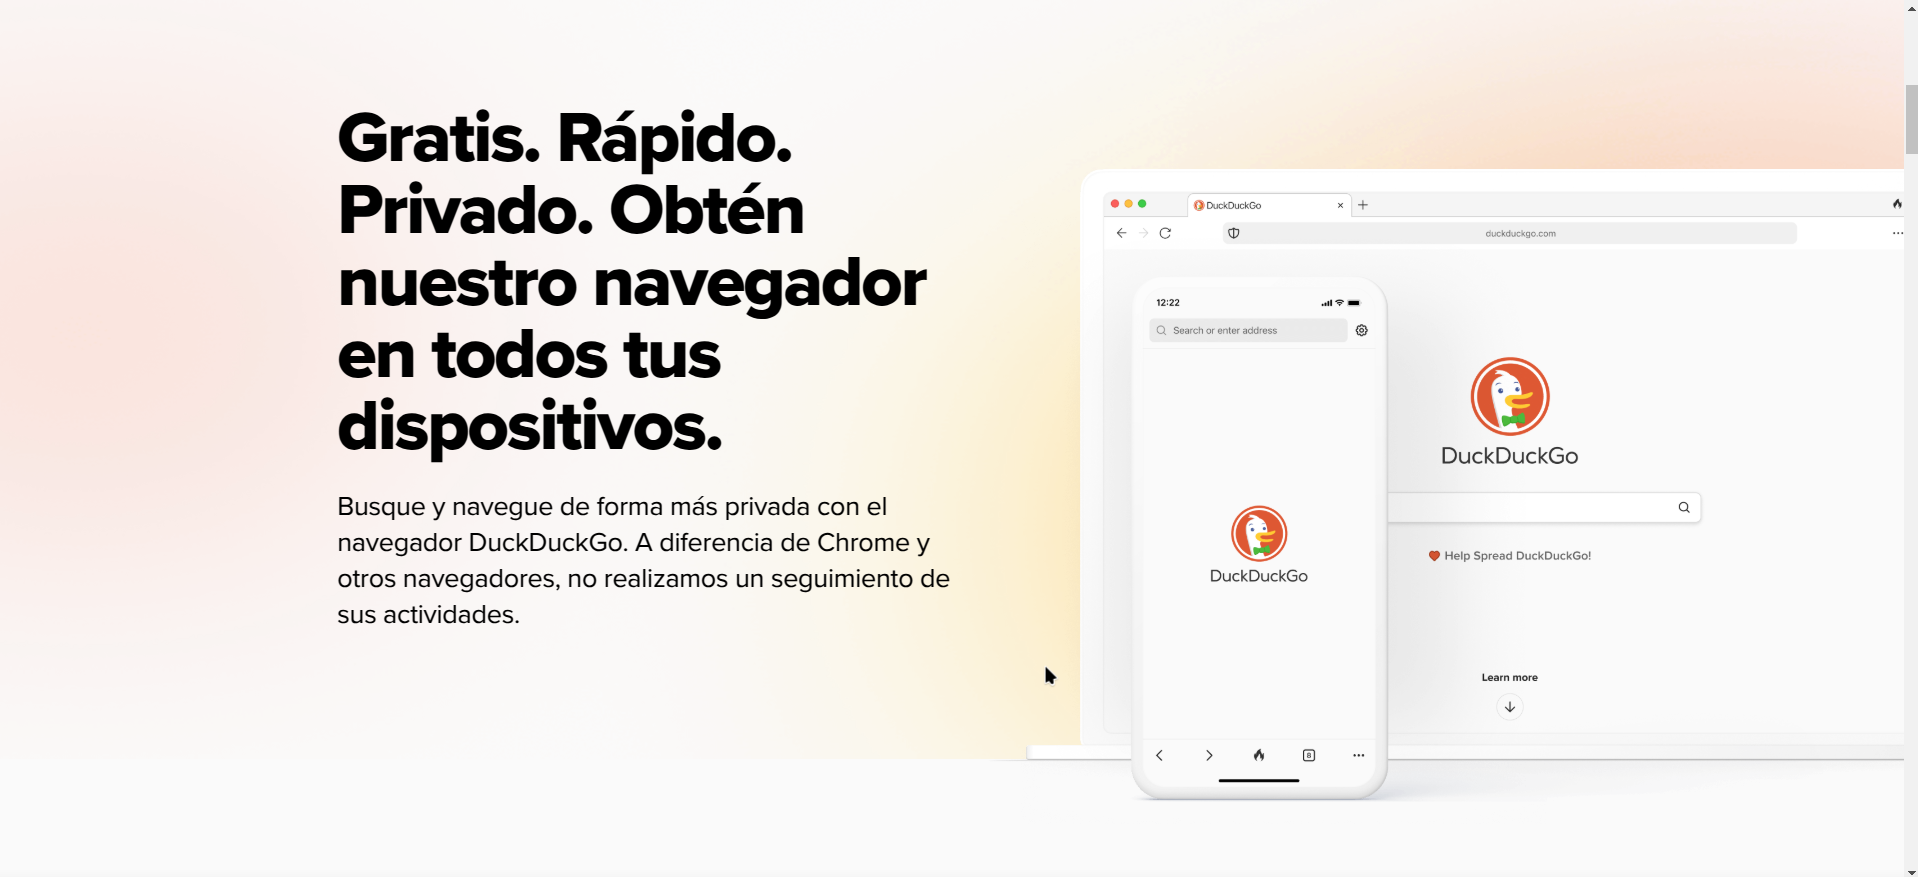
\includegraphics[width=1\linewidth]{images/image05}
	\end{figure}
\end{frame}

\section{Fuentes de Información}

\begin{frame}{Fuentes a Evitar como Referencias Bibliográficas}

	\begin{columns}
		\column{0.5\textwidth}
		\begin{itemize}
			\item Monografias.com
			\item Wikipedia
			\item El Rincón del Vago
			\item Buenas Tareas
			\item \emph{Y otros sitios similares que carecen de rigor académico.}
		\end{itemize}
		\column{0.5\textwidth}
		\begin{figure}[H]
			\centering
			
\includegraphics[width=1\linewidth]{images/image06}
		\end{figure}
	\end{columns}

\end{frame}

\begin{frame}{¿Por qué no Wikipedia?}
	\begin{itemize}
		\item Editada por usuarios sin necesariamente verificación de expertos.
		\item Información puede ser sesgada o no actualizada.
		\item No apta para trabajos académicos que requieren fuentes verificables.
	\end{itemize}

	\begin{figure}[H]
		\centering
		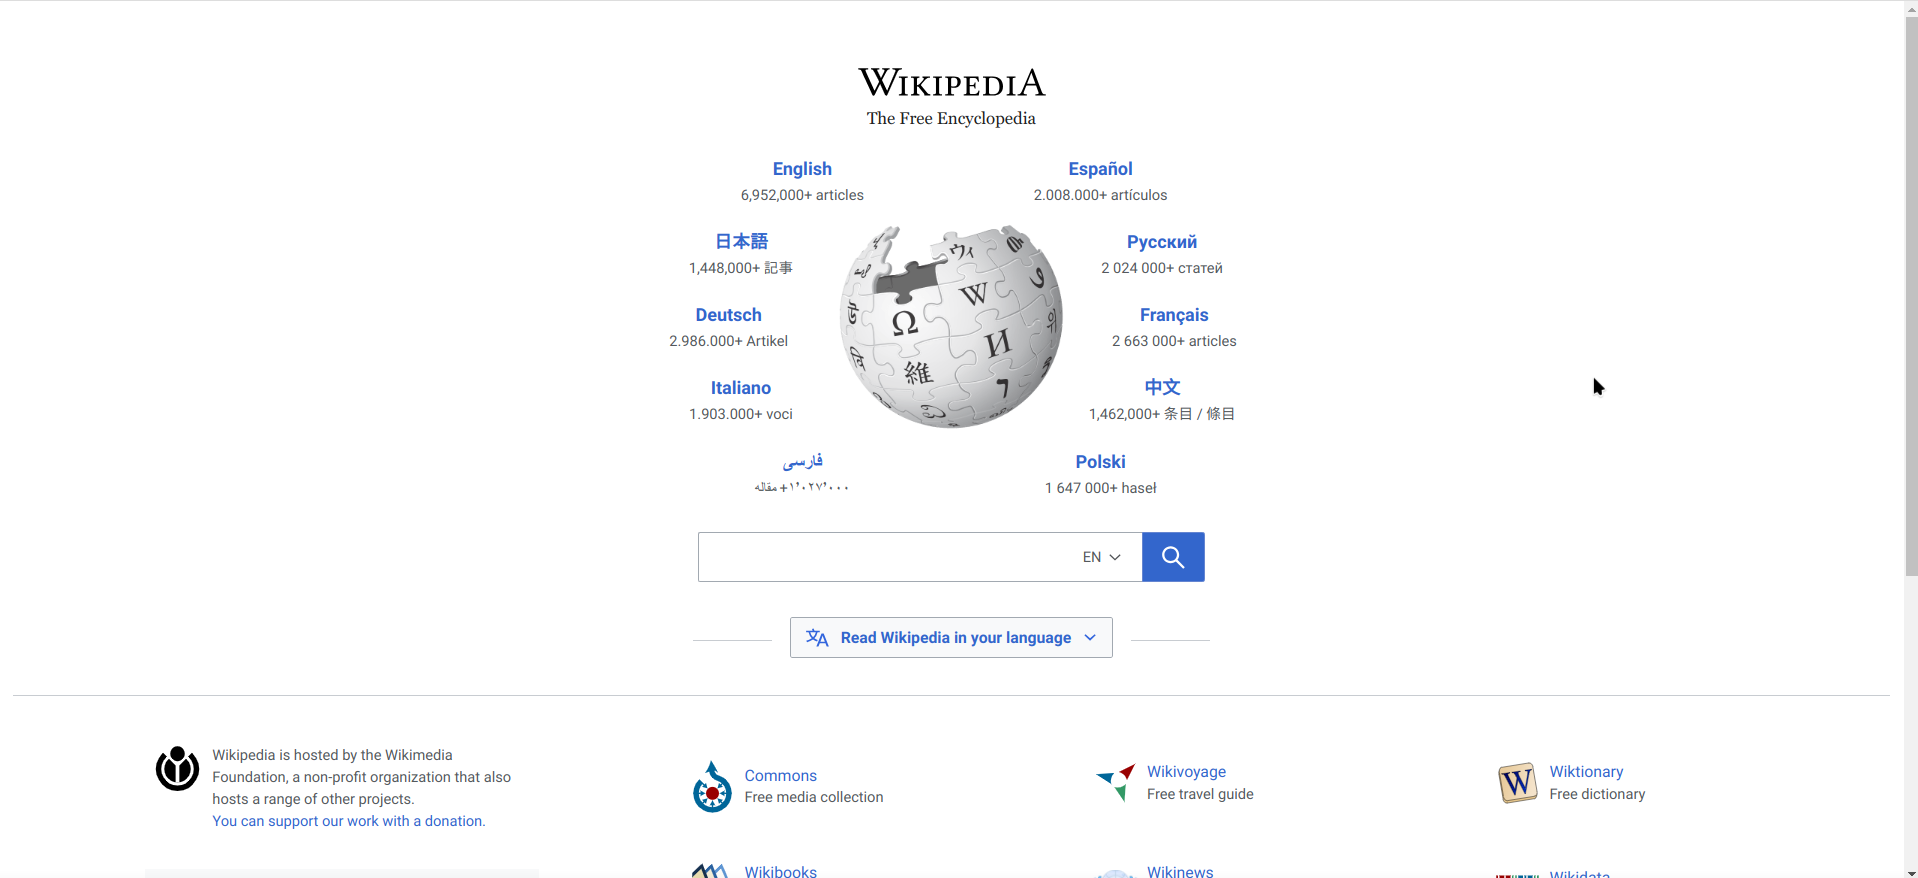
\includegraphics[width=1\linewidth]{images/image07}
	\end{figure}
\end{frame}

\section{Criterios para Evaluar la Calidad y Fiabilidad de la Información}

\begin{frame}{Criterios de Evaluación}
	\begin{description}
		\item[Autoría] ¿Quién es el autor? ¿Es experto o conocido?
		\item[Credenciales] ¿A qué institución pertenece el autor?
		\item[Imparcialidad y Verificación] ¿Es el mensaje objetivo? ¿Se verifica la información?
		\item[Vigencia] ¿La información está actualizada?
	\end{description}
\end{frame}

\begin{frame}{Extensiones Populares}
	\begin{table}
		\centering
		\resizebox{\textwidth}{!}{%
			\begin{tabular}{lll}
				\toprule
				\textbf{Dominio Corto} & \textbf{Descripción} & \textbf{Uso}                                                  \\
				\midrule
				.com                   & Comercial            & Sitios de negocios                                            \\
				.org                   & Organización         & Entidades sin ánimo de lucro                                  \\
				.edu                   & Educativo            & Instituciones educativas como universidades, colegios         \\
				.gov                   & Gobierno             & Sitios oficiales del gobierno                                 \\
				.net                   & Network              & Se utiliza comúnmente para diversas empresas u organizaciones \\
				.pe                    & País                 & Indica la relación del sitio web con el país                  \\
				\bottomrule
			\end{tabular}
		}
	\end{table}
\end{frame}

\section{Principios Básicos para una Búsqueda}

\begin{frame}{Dónde Buscar}
	\begin{itemize}
		\item Google Académico
		\item WolframAlpha
		\item Creative Commons Search
	\end{itemize}
\end{frame}

\section{Observaciones en Búsquedas}

\begin{frame}{Búsquedas Simples}
	\begin{block}{Características}
		\begin{itemize}
			\item \alert{Omisión de preposiciones}: ``el'', ``la'', ``y'', ``de'', etc.
			\item \alert{Orden de palabras}: No importa el orden de las palabras.
			\item \alert{Mayúsculas y minúsculas}: No se distingue entre mayúsculas y minúsculas.
			\item \alert{Acentos}: No se distinguen los acentos.
		\end{itemize}
	\end{block}
	\begin{exampleblock}{Ejemplo}
		\begin{itemize}
			\item Búsqueda: ``libro historia''
			\item Resultados: ``Historia del libro'', ``Libro de historia'', etc.
		\end{itemize}
	\end{exampleblock}
\end{frame}

\begin{frame}{Búsquedas Avanzadas}
	\begin{block}{Características}
		\begin{itemize}
			\item \alert{Mayúsculas y minúsculas}: No se distinguen.
			\item \alert{Caracteres especiales y puntuación}: @ \# \$ \% \& * ( ) = + [ ] \. son ignorados.
		\end{itemize}
	\end{block}

	\begin{alertblock}{Operadores Avanzados}
		\begin{itemize}
			\item \textbf{Frase exacta}: ``librería'' o +librería
			\item \textbf{Con alguna palabra}: emelec 2015 OR 2016 o emelec 2015 | 2016
			\item \textbf{Excluyente}: \texttt{Terremoto -víctimas}
		\end{itemize}
	\end{alertblock}

	\begin{exampleblock}{Ejemplos}
		\begin{itemize}
			\item ``crisis económica en Perú'' - Busca exactamente esa frase.
			\item emelec 2015 | 2016 - Encuentra resultados de cualquier año.
		\end{itemize}
	\end{exampleblock}
\end{frame}

\begin{frame}{Operadores Booleanos}
	\begin{block}{Uso de Operadores}
		\begin{description}
			\item[\texttt{OR}]
			      Busca páginas con al menos una palabra. Ejemplo: \alert{crisis OR depresión}
			\item[\texttt{AND}]
			      Busca páginas con ambas palabras. Ejemplo: \alert{crisis AND económica}
			\item[\texttt{-}]
			      Excluye páginas con el término. Ejemplo: \alert{crisis -económica}, \alert{jaguar velocidad -motor}
			\item[\texttt{+}]
			      Incluye páginas con el término exacto. Ejemplo: \alert{cursos pintura +óleo}
			\item[`` '']
			      Muestra páginas con la frase exacta. Ejemplo: \alert{``crisis económica en Perú''}
		\end{description}
	\end{block}

\end{frame}

\begin{frame}
	\frametitle{Introducción a los Comandos de Búsqueda}
	\begin{itemize}
		\item Los motores de búsqueda ofrecen comandos para refinar nuestras búsquedas.
		\item Aprender estos comandos puede mejorar significativamente la calidad y
		      relevancia de los resultados.
	\end{itemize}
\end{frame}

\begin{frame}
	\frametitle{Uso de Comillas ""}
	\textbf{Descripción:}
	\begin{itemize}
		\item Busca la frase exacta entre comillas.
	\end{itemize}
	\begin{exampleblock}{Ejemplos:}
		\begin{itemize}
			\item \textbf{``metodología investigación cualitativa''} - Esto buscaría la frase exacta en los resultados
			\item \textbf{``impacto cambio climático agricultura''}
			\item \textbf{``educación virtual tiempos pandemia''}
		\end{itemize}
	\end{exampleblock}

\end{frame}

\begin{frame}
	\frametitle{Operador AND}
	\textbf{Descripción:}
	\begin{itemize}
		\item Combina términos; ambos deben estar presentes en los resultados.
	\end{itemize}
	\begin{exampleblock}{Ejemplos:}
		\begin{itemize}
			\item \textbf{covid AND perú} - Busca documentos que contengan ambas palabras.
			\item \textbf{educación AND tecnología} - Busca documentos que mencionen ambos términos.
			\item \textbf{sostenibilidad AND desarrollo} - Ambos términos deben aparecer en los resultados.
		\end{itemize}
	\end{exampleblock}
\end{frame}

\begin{frame}
	\frametitle{Operador OR}
	\textbf{Descripción:}
	\begin{itemize}
		\item Busca uno u otro término; al menos uno debe estar presente.
	\end{itemize}
	\begin{exampleblock}{Ejemplos:}
		\begin{itemize}
			\item monografía OR tesis - Busca páginas que tengan cualquiera de los dos términos.
			\item criptomonedas OR criptodivisas
		\end{itemize}
	\end{exampleblock}

\end{frame}

\begin{frame}
	\frametitle{Exclusión de Términos (-)}
	\textbf{Descripción:}
	\begin{itemize}
		\item Excluye resultados que contengan el término especificado después del signo
		      menos.
	\end{itemize}

	\begin{exampleblock}{Ejemplos:}
		\begin{itemize}
			\item \textbf{investigación -comercial} - Esto excluiría resultados que mencionen ``comercial''.
			\item \textbf{tecnología -militar} - Esto excluiría resultados que mencionen ``militar''.
			\item \textbf{critomonedas -bitcoins - bitcoin}
		\end{itemize}
	\end{exampleblock}

\end{frame}

\begin{frame}
	\frametitle{Inclusión Forzosa (+)}
	\textbf{Descripción:}
	\begin{itemize}
		\item Asegura que el término especificado después del signo más esté incluido.
	\end{itemize}

	\begin{exampleblock}{Ejemplos:}
		\begin{itemize}
			\item \textbf{investigación +universidad }- Asegura que ``universidad'' esté en los resultados.
			\item \textbf{salud +mental} - Garantiza que ``mental'' aparezca en los resultados sobre salud.
		\end{itemize}
	\end{exampleblock}
\end{frame}

\begin{frame}
	\frametitle{Rango de Números (..)}
	\textbf{Descripción:}
	\begin{itemize}
		\item Busca resultados dentro de un rango numérico específico.
	\end{itemize}

	\begin{exampleblock}{Ejemplos:}
		\begin{itemize}
			\item violencia sociopolítica 1980..2002 AND perú
		\end{itemize}
	\end{exampleblock}

\end{frame}

\begin{frame}
	\frametitle{Tipo de Documento (filetype:)}
	\textbf{Descripción:}
	\begin{itemize}
		\item Filtra resultados según el tipo de archivo.
	\end{itemize}
	\begin{exampleblock}{Ejemplos:}
		\begin{itemize}
			\item \textbf{expotaciones filetype:pdf} - Busca exportaciones en formato PDF.
			\item \textbf{expotaciones perú filetype:xlsx} - Busca exportaciones en formato XLSX.
		\end{itemize}
	\end{exampleblock}

\end{frame}

\begin{frame}
	\frametitle{Búsqueda en el Texto (allintext:, intext:)}
	\textbf{Descripción:}
	\begin{itemize}
		\item Busca palabras específicas dentro del texto de la página.
	\end{itemize}

	\begin{exampleblock}{Ejemplos:}
		\begin{itemize}
			\item \textbf{allintext:metodología cuantitativa} - Todas las palabras deben estar en el texto de la página.
			\item \textbf{intext:cuantitativo} - Busca páginas que contengan "cuantitativo" en su texto.
		\end{itemize}
	\end{exampleblock}

\end{frame}

\begin{frame}
	\frametitle{Búsqueda en el Título (allintitle:, intitle:)}
	\textbf{Descripción:}
	\begin{itemize}
		\item Busca palabras en el título del documento o página.
	\end{itemize}

	\begin{exampleblock}{Ejemplos:}
		\begin{itemize}
			\item \textbf{allintitle:tesis doctoral} - Todas las palabras deben estar en el título.
			\item \textbf{intitle:tesis} - Busca páginas con "tesis" en el título.
		\end{itemize}
	\end{exampleblock}
\end{frame}

\begin{frame}
	\frametitle{Caracteres Wildcard (*)}
	\textbf{Descripción:}
	\begin{itemize}
		\item Sustituye palabras o partes de palabras en la búsqueda.
	\end{itemize}
	\textbf{Ejemplo:}
	\begin{itemize}
		\item "investigación en *" - Busca frases que empiecen con "investigación en".
	\end{itemize}
\end{frame}

\begin{frame}
	\frametitle{Combinación de Comandos}
	\textbf{Descripción:}
	\begin{itemize}
		\item Mezcla varios comandos para una búsqueda más precisa.
	\end{itemize}
	\begin{exampleblock}{Ejemplos:}
		\begin{itemize}
			\item \textbf{intitle:tesis filetype:pdf site:.edu ``metodología cualitativa'' -cuantitativa} - Busca tesis en formato PDF de sitios .edu con ``metodología cualitativa'' en el título y excluye ``cuantitativa''.
			\item \textbf{allintext:desarrollo sostenible site:.org -2020} - Busca páginas en organizaciones sin fines de lucro que mencionen ``desarrollo sostenible'' en el texto, pero excluyendo resultados del año 2020.
		\end{itemize}
	\end{exampleblock}
\end{frame}

% Sección 9
\section{Tablas, Figuras y Notas}

\begin{frame}
	\frametitle{Objetivo de la sesión}
	Al finalizar la sesión, las y los participantes conocerán cómo presentar tablas y figuras de distintos tipos, según el estilo APA 7a edición.
\end{frame}

\begin{frame}
	\frametitle{Estilo APA para principiantes: tablas y figuras}
	\begin{itemize}
		\item Tablas y figuras: ¿qué son y por qué usarlas?
		\item ¿Cómo presentar tablas y figuras según el estilo APA?
		\item ¿Cómo presentar tablas y figuras tomadas de una fuente?
		\item ¿Cómo presentar tablas y figuras de elaboración propia?
		\item ¿Cómo realizar llamados a tablas y figuras en el texto?
		\item Ejemplos en vivo de corrección de tablas y figuras en el estilo APA
	\end{itemize}
\end{frame}

\begin{frame}
	\frametitle{¿Qué es una tabla? ¿Qué es una figura? ¿Por qué usarlas?}

	\begin{columns}[c] % The "c" option specifies centered vertical alignment while the "t" option is used for top vertical alignment
		\begin{column}{0.2\textwidth} % Left column width
			\textbf{¿Por qué usar tablas o figuras?}
		\end{column}
		\begin{column}{0.5\textwidth} % Right column width
			\begin{itemize}
				\item Permiten \colorbox{yellow}{presentar gran cantidad de información}
				      \colorbox{yellow}{de manera eficiente} y hacer tus datos más comprensibles.
				\item Pueden \colorbox{yellow}{resumir la información}, para presentar resultados,
				      estimar alguna estadística o comparar datos.
				\item No deben usarse como algo decorativo en un texto académico,
				      \colorbox{yellow}{deben tener un propósito claro.}
			\end{itemize}
		\end{column}
	\end{columns}

\end{frame}

\begin{frame}
	\frametitle{Tabla y Figura}

	\begin{columns}[c] % The "c" option specifies centered vertical alignment while the "t" option is used for top vertical alignment
		\begin{column}{0.5\textwidth} % Left column width
			\textbf{Tabla}

			Las tablas muestran valores numéricos o información en formato texto dispuestos
			en columnas y filas.
			\begin{figure}[H]
				\centering
				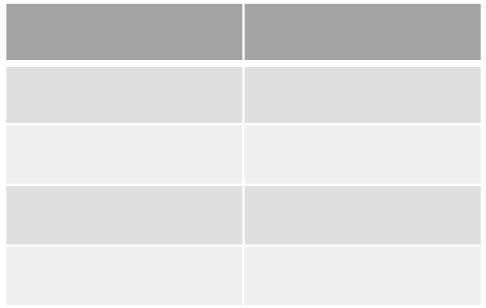
\includegraphics[width=1\linewidth]{images/screenshot001}
			\end{figure}
		\end{column}
		\begin{column}{0.5\textwidth} % Right column width
			\textbf{Figura}

			Una figura puede ser cualquier tipo de ilustración o representación no textual
			que no sea una tabla.
			\begin{itemize}
				\item Gráfico estadístico
				\item Fotografía
				\item Diagrama
				\item Dibujo
				\item Cualquier representación visual no textual
			\end{itemize}
		\end{column}
	\end{columns}

\end{frame}

\begin{frame}
	\frametitle{Tabla y Figura}

	\begin{columns}[c] % The "c" option specifies centered vertical alignment while the "t" option is used for top vertical alignment
		\begin{column}{0.5\textwidth} % Left column width
			\textbf{Tabla}
			\begin{figure}
				\centering
				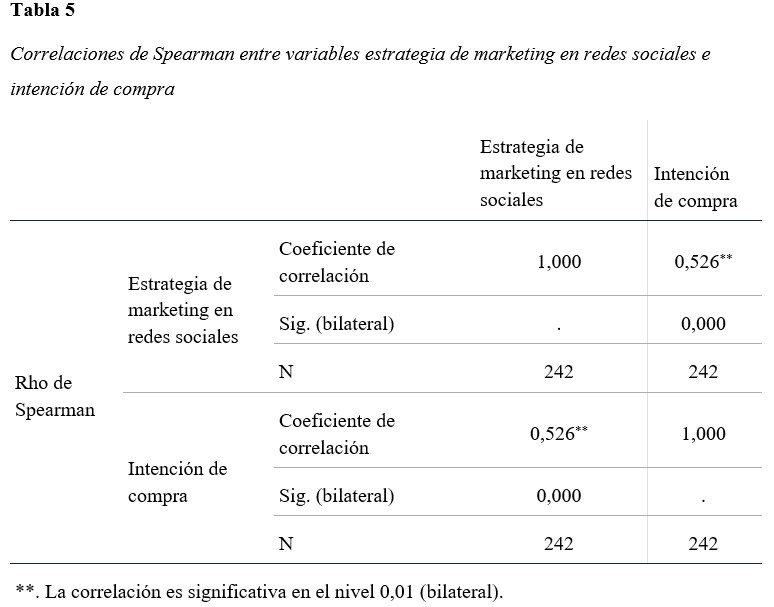
\includegraphics[width=1\linewidth]{images/screenshot002}
			\end{figure}

		\end{column}
		\begin{column}{0.5\textwidth} % Right column width
			\textbf{Figura}

			\begin{figure}
				\centering
				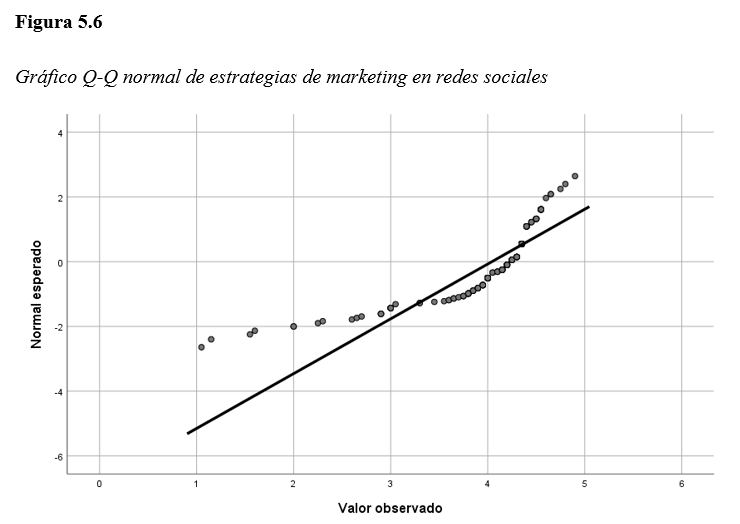
\includegraphics[width=1\linewidth]{images/screenshot003}
			\end{figure}

		\end{column}
	\end{columns}

\end{frame}

\begin{frame}
	\frametitle{¿Cómo presentar una tabla?}

	\begin{columns}[c] % The "c" option specifies centered vertical alignment while the "t" option is used for top vertical alignment
		\begin{column}{0.5\textwidth} % Left column width
			\begin{figure}[H]
				\centering
				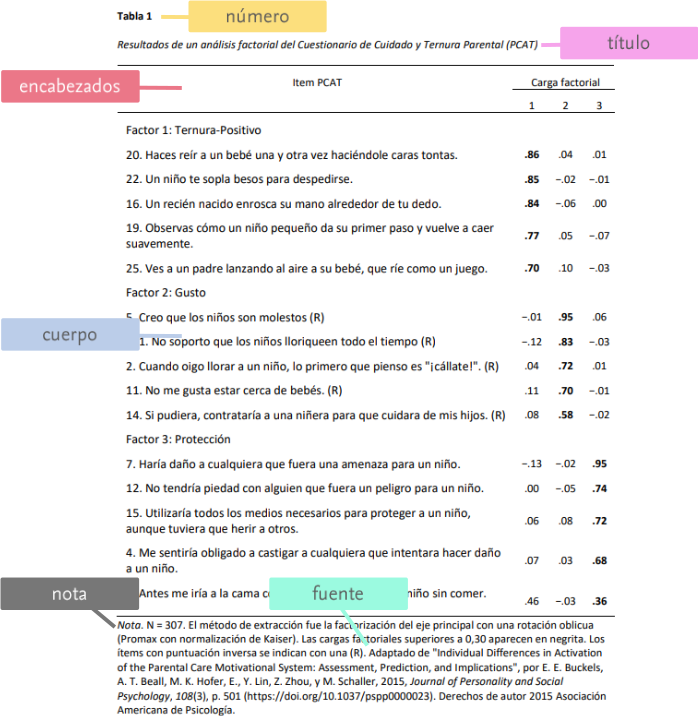
\includegraphics[width=1\linewidth]{images/screenshot004}
			\end{figure}
		\end{column}
		\begin{column}{0.5\textwidth} % Right column width
			\scriptsize
			\begin{itemize}
				\item \textbf{Número}: Aparece arriba de la tabla y en negrita.
				\item \textbf{Título}: Breve pero descriptivo. Aparece debajo del número, a doble espacio, en mayúscula de oración y en cursiva.
				\item \textbf{Encabezados}: Todas las tablas deben incluir encabezados de columnas.
				\item \textbf{Cuerpo}: Incluye todas las filas y columnas de una tabla. Puede estar a un espacio, espacio y medio o doble espacio.
				\item \textbf{Nota}: Aparece debajo de la tabla, puede ser general, específica o de probabilidad, de ser el caso. Describe el contenido de la tabla que no puede entenderse.
				\item \textbf{Fuente}: Indicar la fuente de la tabla, de ser el caso.
			\end{itemize}

		\end{column}
	\end{columns}

\end{frame}

\begin{frame}
	\frametitle{¿Cómo presentar una figura?}

	\begin{columns}[c] % The "c" option specifies centered vertical alignment while the "t" option is used for top vertical alignment
		\begin{column}{0.5\textwidth} % Left column width
			\begin{figure}
				\centering
				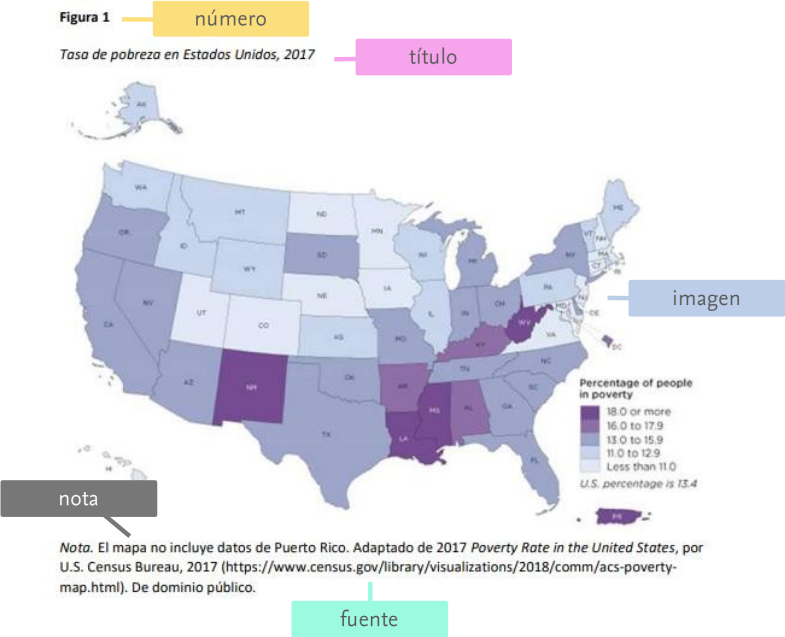
\includegraphics[width=1\linewidth]{images/screenshot005}
			\end{figure}

		\end{column}
		\begin{column}{0.5\textwidth} % Right column width
			\scriptsize
			\begin{itemize}
				\item \textbf{Número}: Aparece arriba de la figura y en negrita.
				\item \textbf{Título}: Breve pero descriptivo. Aparece debajo del número, a doble espacio, en mayúscula de oración y en cursiva.
				\item \textbf{Imagen}: Es la propia gráfica, diagrama, dibujo, mapa, fotografía u otra ilustración.
				\item \textbf{Nota}: Aparece debajo de la imagen. Describe el contenido de la figura que no puede entenderse a partir del título e imagen.
				\item \textbf{Fuente}: Indicar la fuente de la figura, de ser el caso.
			\end{itemize}

		\end{column}
	\end{columns}

\end{frame}

\begin{frame}
	\frametitle{¿Cómo presentar una figura?}

	\begin{columns}[c] % The "c" option specifies centered vertical alignment while the "t" option is used for top vertical alignment
		\begin{column}{0.5\textwidth} % Left column width
			\textbf{¿Cómo presentar tablas y figuras tomadas de una fuente?}
		\end{column}
		\begin{column}{0.5\textwidth} % Right column width
			\begin{itemize}
				\item \textbf{Reimpresión}: Cuando utilizas exactamente y sin ningún cambio la tabla o figura encontrada en una fuente, usa el término "De" en la Nota.
				\item \textbf{Adaptación}: Cuando utilizas una tabla o figura encontrada en una fuente de información, pero haciéndole modificaciones, usa la expresión "Adaptada de" en la Nota.
			\end{itemize}

		\end{column}
	\end{columns}

\end{frame}

\begin{frame}{Estilos}
	\frametitle{¿Cómo atribuir la fuente de una figura o tabla?}
	\begin{figure}
		\centering
		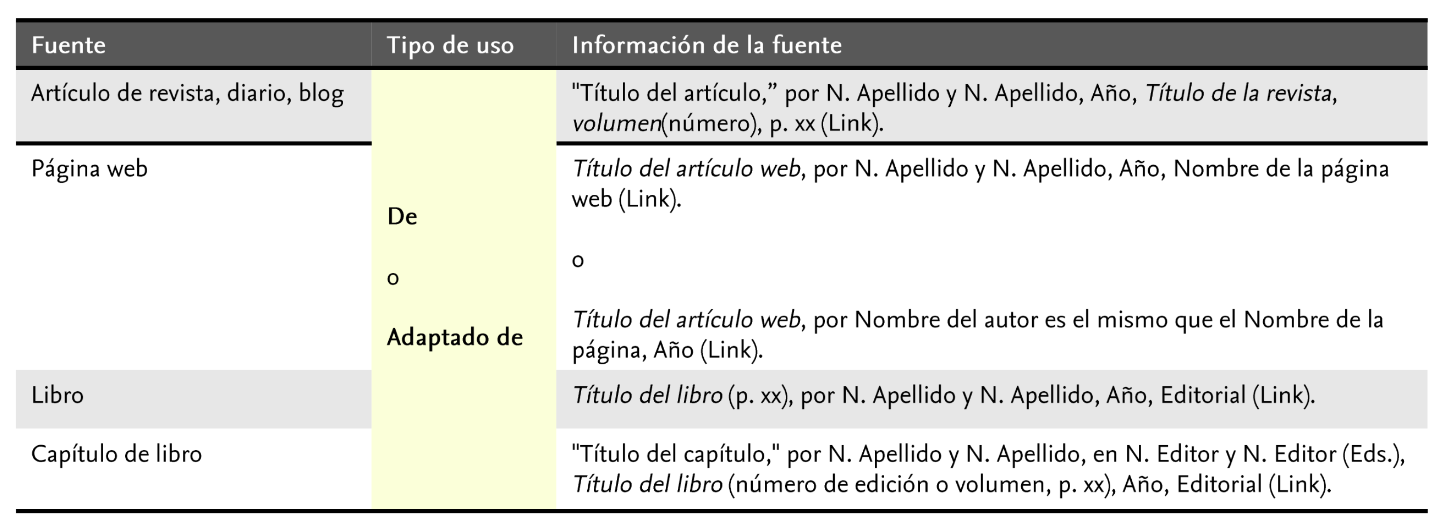
\includegraphics[width=1\linewidth]{images/screenshot006}
	\end{figure}

	Para otros tipos de publicaciones, proporciona el título, autor, año y fuente
	de información

\end{frame}

\begin{frame}
	\frametitle{Figura tomada de un libro}

	\begin{columns}[c] % The "c" option specifies centered vertical alignment while the "t" option is used for top vertical alignment
		\begin{column}{0.5\textwidth} % Left column width
			\begin{figure}
				\centering
				
\includegraphics[width=0.5\linewidth]{images/screenshot007}
			\end{figure}
			\scriptsize{

				Título: Fundamentos de marketing

				Autor: Gary Armstrong y Philip Kotler

				Editorial: Pearson

				Año: 2013}

		\end{column}
		\begin{column}{0.5\textwidth} % Right column width
			\begin{figure}
				\centering
				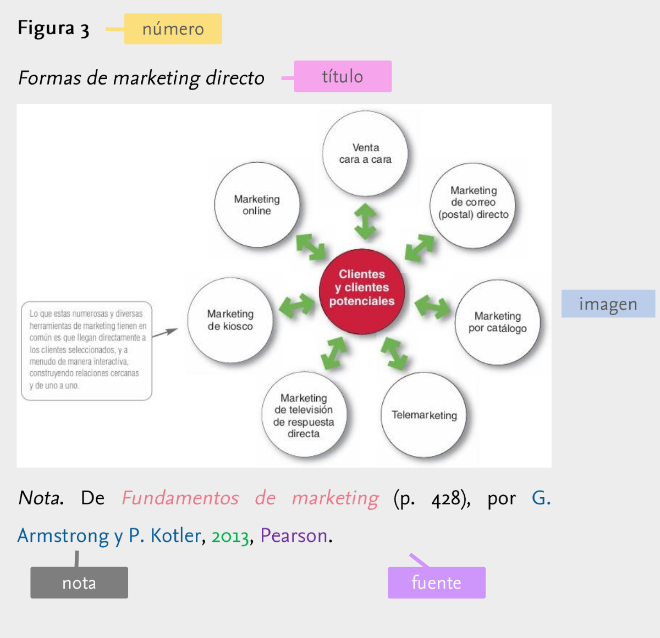
\includegraphics[width=1\linewidth]{images/screenshot008}
			\end{figure}

		\end{column}
	\end{columns}

\end{frame}

\begin{frame}
	\frametitle{Figura tomada de un libro}

	\begin{columns}[c] % The "c" option specifies centered vertical alignment while the "t" option is used for top vertical alignment
		\begin{column}{0.5\textwidth} % Left column width
			\begin{figure}
				\centering
				
\includegraphics[width=0.3\linewidth]{images/screenshot009}
			\end{figure}

			\scriptsize{
				Título: Violencia y autoritarismo en ele Perú: Bajo la sombra de Sendero y la dictadura de Fujimori

				Autor: Jo-Marie Burt

				Editorial: Instituto de Estudios Peruanos

				Año: 2011

				Link: https://repositorio.iep.or.pe/handle/IEP/1216}

		\end{column}
		\begin{column}{0.5\textwidth} % Right column width
			\begin{figure}
				\centering
				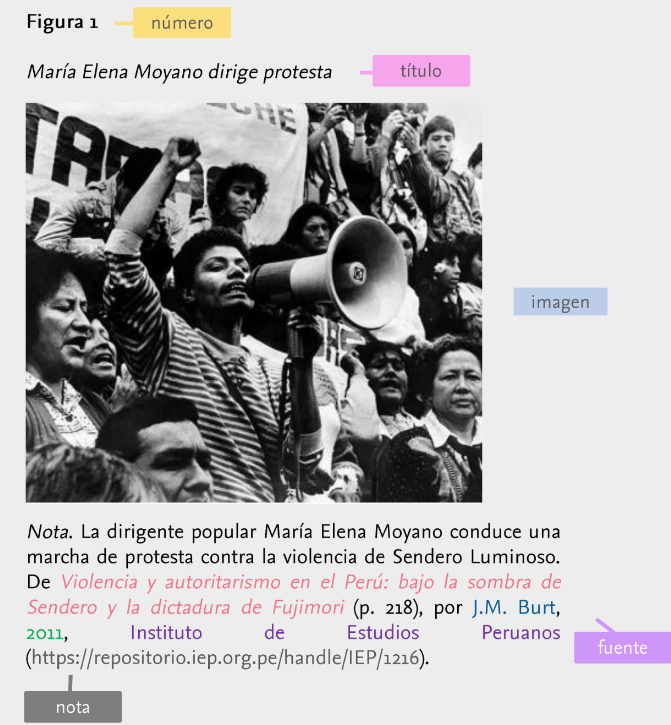
\includegraphics[width=1\linewidth]{images/screenshot010}
			\end{figure}

		\end{column}
	\end{columns}

\end{frame}

\begin{frame}
	\frametitle{Figura tomada de una página web}

	\begin{columns}[c] % The "c" option specifies centered vertical alignment while the "t" option is used for top vertical alignment
		\begin{column}{0.5\textwidth} % Left column width
			\begin{figure}
				\centering
				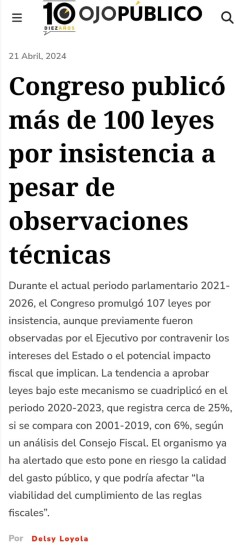
\includegraphics[width=0.2\linewidth]{images/screenshot011}
			\end{figure}
			\scriptsize{

				Título del articulo: Congreso publicó más de 100 leyes por insistencia a pesar
				de observaciones técnicas

				Autor: Delsy Loyola

				Editorial: Ojo Público

				Año: 2024

				Link:
				https://ojo-publico.com/politica/congreso-publico-mas-de-100-leyes-por-insistencia-pesar-alertas}

		\end{column}
		\begin{column}{0.5\textwidth} % Right column width
			\begin{figure}
				\centering
				
\includegraphics[width=1\linewidth]{images/screenshot012}
			\end{figure}

		\end{column}
	\end{columns}

\end{frame}

\begin{frame}
	\frametitle{Tabla tomada de un artículo científico}

	\begin{columns}[c] % The "c" option specifies centered vertical alignment while the "t" option is used for top vertical alignment
		\begin{column}{0.5\textwidth} % Left column width
			\begin{figure}
				\centering
				
\includegraphics[width=0.4\linewidth]{images/screenshot014}
			\end{figure}
			\scriptsize{

				Título del articulo: ¿Cuánto apoyan los peruanos las creencias de conspiración
				sobre las vacunas contra la COVID-19?

				Autor: Tomás Caycho-Rodríguez, Miguel Gallegos, Pablo D. Valencia y Lindsey W.
				Vilca

				Revista: Atención Primaria, 54(5), 1-3

				Año: 2022 Link: https://doi.org/10.1016/j.aprim.2022.102318 }

		\end{column}
		\begin{column}{0.5\textwidth} % Right column width
			\begin{figure}
				\centering
				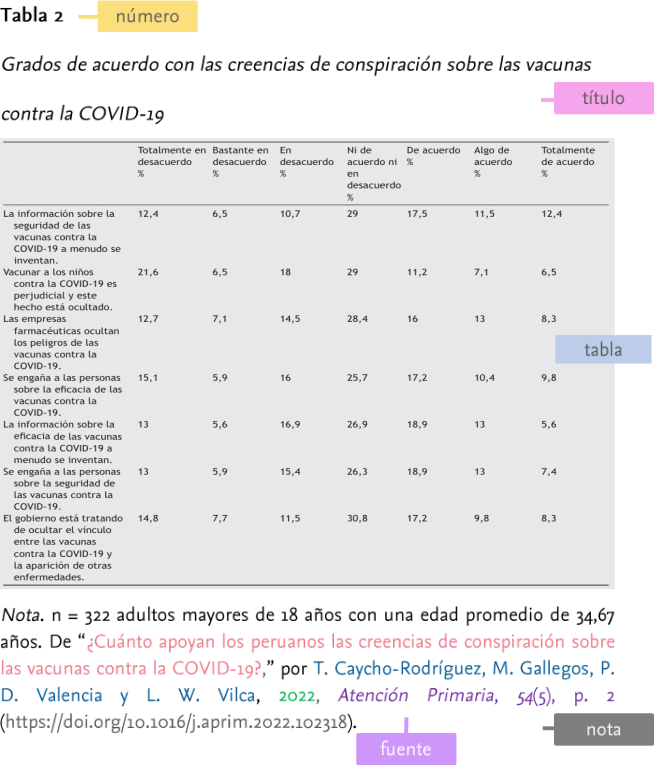
\includegraphics[width=0.9\linewidth]{images/screenshot013}
			\end{figure}

		\end{column}
	\end{columns}

\end{frame}

\begin{frame}
	\frametitle{Figura tomada de un artículo científico}

	\begin{columns}[c] % The "c" option specifies centered vertical alignment while the "t" option is used for top vertical alignment
		\begin{column}{0.5\textwidth} % Left column width
			\begin{figure}
				\centering
				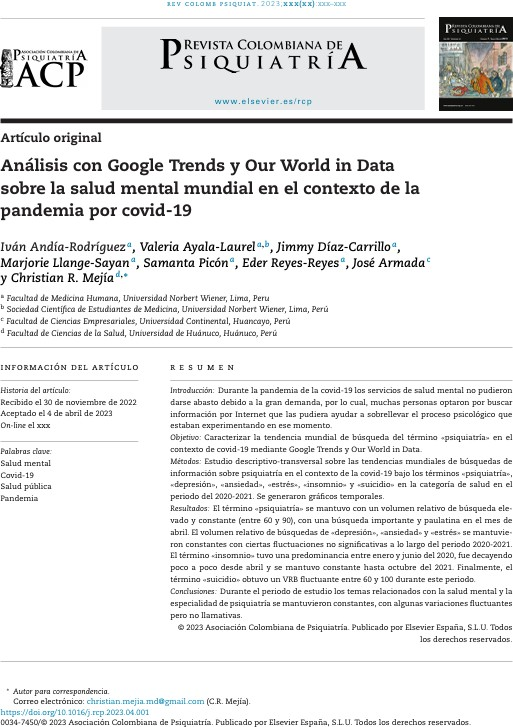
\includegraphics[width=0.4\linewidth]{images/screenshot016}
			\end{figure}
			\scriptsize{

				Artículo: Análisis con Google Trends y Our World in Data sobre la salud mental
				mundial en el contexto de la pandemia por covid-19

				Autor: Iván Andía-Rodríguez, Valeria Ayala-Laurel, Jimmy Díaz-Carrillo,
				Marjorie Llange-Sayan, Samanta Picón, Eder Reyes-Reyes, José Armada y Christian
				R. Mejía

				Revista: Revista Colombiana de Psiquiatría, 52(1), 1-7

				Año: 2023

				Link: https://doi.org/10.1016/j.rcp.2023.04.001 }

		\end{column}
		\begin{column}{0.5\textwidth} % Right column width
			\begin{figure}
				\centering
				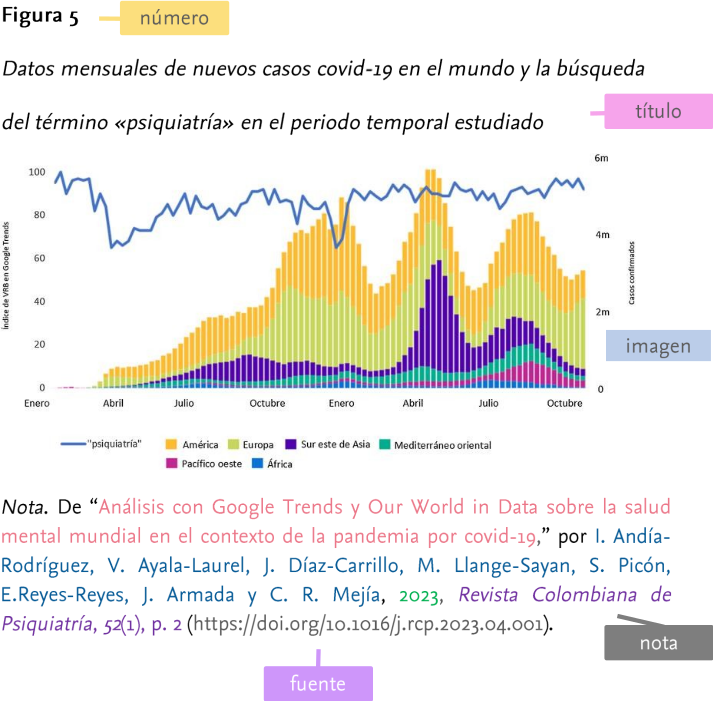
\includegraphics[width=0.9\linewidth]{images/screenshot015}
			\end{figure}

		\end{column}
	\end{columns}

\end{frame}

\begin{frame}
	\frametitle{Figura tomada de un artículo científico}

	\begin{columns}[c] % The "c" option specifies centered vertical alignment while the "t" option is used for top vertical alignment
		\begin{column}{0.5\textwidth} % Left column width
			\begin{figure}
				\centering
				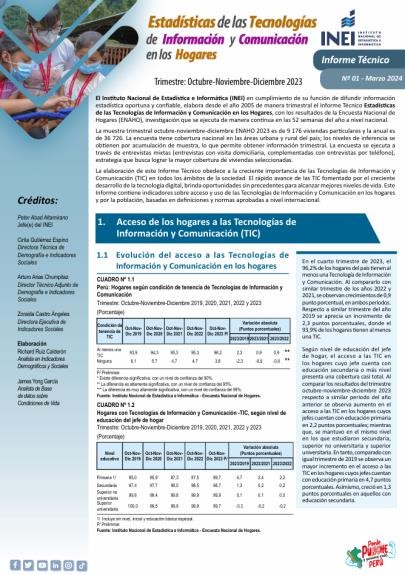
\includegraphics[width=0.4\linewidth]{images/screenshot018}
			\end{figure}
			\scriptsize{

				Título: Las tecnologías de información y comunicación en los hogares:
				oct-nov-dic 2023

				Autor: Instituto Nacional de Estadística e Informática

				Año: 2024

				Página: Instituto Nacional de Estadística e Informática

				Link:
				https://www.gob.pe/institucion/inei/informes-publicaciones/5408920-las-tecnologias-de-informacion-y-comunicacion-en-los-hogares-oct-nov-dic-2023
			}

		\end{column}
		\begin{column}{0.5\textwidth} % Right column width
			\begin{figure}
				\centering
				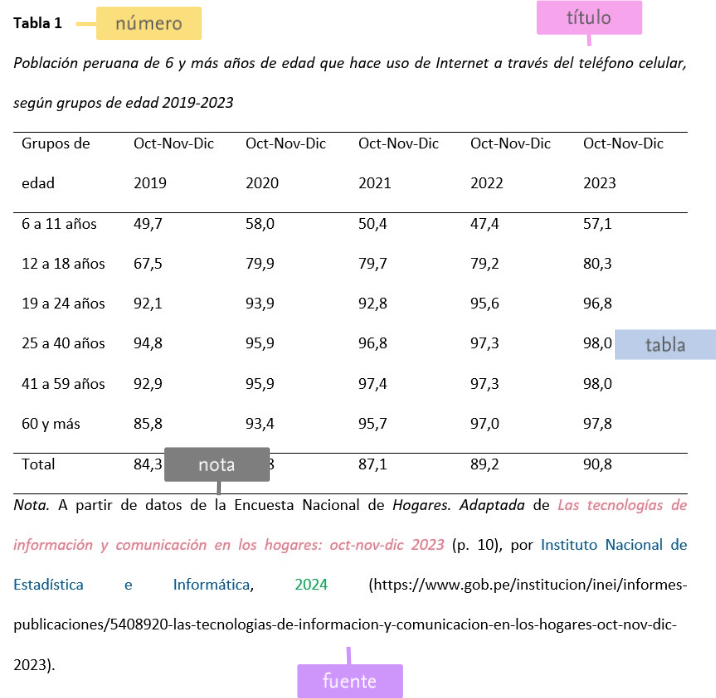
\includegraphics[width=0.9\linewidth]{images/screenshot017}
			\end{figure}

		\end{column}
	\end{columns}

\end{frame}

\begin{frame}{¿Cómo presentar tablas y figuras de elaboración propia?}
	\begin{figure}
		\centering
		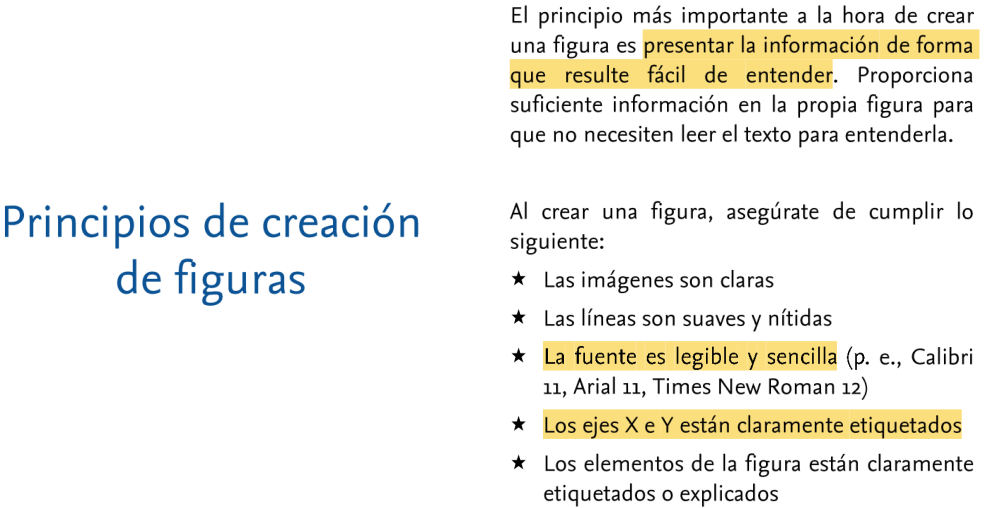
\includegraphics[width=1\linewidth]{images/screenshot019}
	\end{figure}

\end{frame}

\begin{frame}
	\frametitle{Figura tomada de un artículo científico}

	\begin{columns}[c] % The "c" option specifies centered vertical alignment while the "t" option is used for top vertical alignment
		\begin{column}{0.5\textwidth} % Left column width
			Figura de elaboración propia
		\end{column}
		\begin{column}{0.5\textwidth} % Right column width
			\begin{figure}
				\centering
				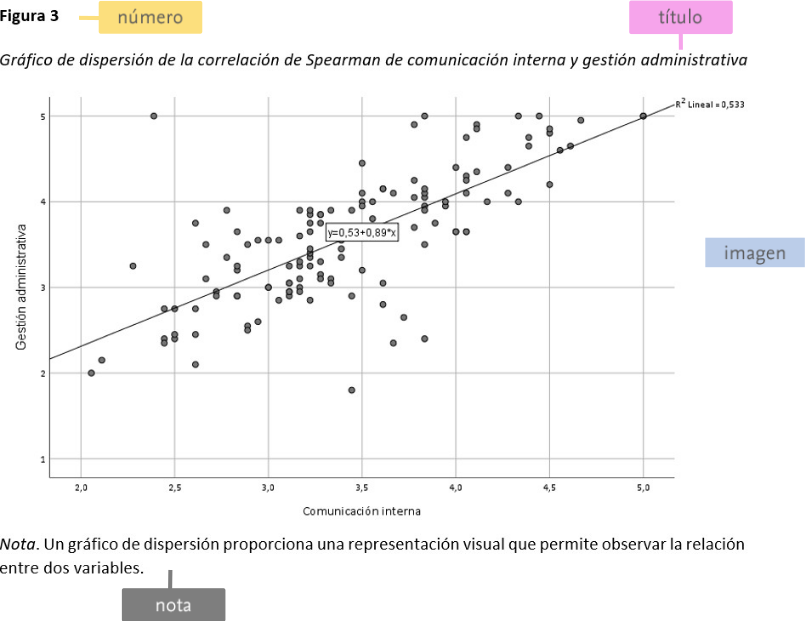
\includegraphics[width=1\linewidth]{images/screenshot020}
			\end{figure}

		\end{column}
	\end{columns}

\end{frame}

\begin{frame}
	\frametitle{Figura tomada de un artículo científico}

	\begin{columns}[c] % The "c" option specifies centered vertical alignment while the "t" option is used for top vertical alignment
		\begin{column}{0.5\textwidth} % Left column width
			Tabla de elaboración propia
		\end{column}
		\begin{column}{0.5\textwidth} % Right column width
			\begin{figure}
				\centering
				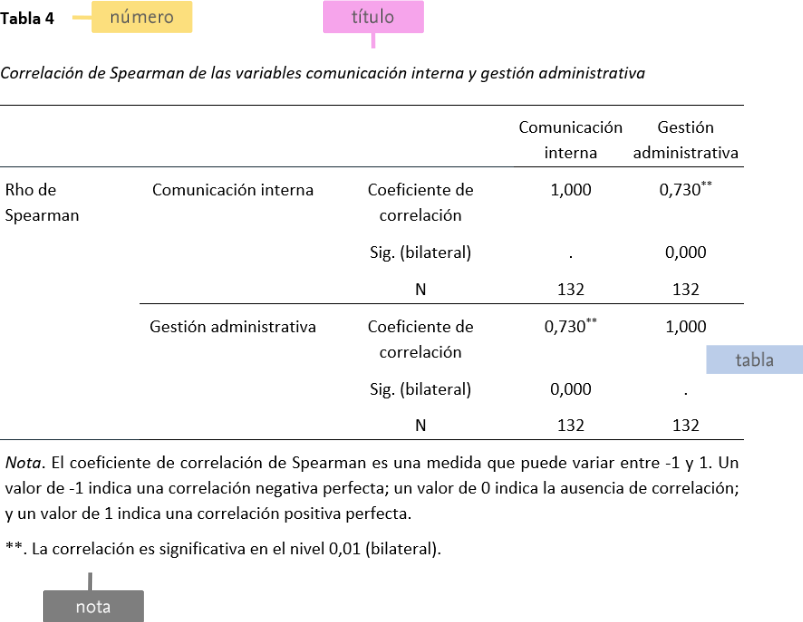
\includegraphics[width=1\linewidth]{images/screenshot021}
			\end{figure}

		\end{column}
	\end{columns}

\end{frame}

\begin{frame}
	\frametitle{Figura tomada de un artículo científico}

	\begin{columns}[c] % The "c" option specifies centered vertical alignment while the "t" option is used for top vertical alignment
		\begin{column}{0.5\textwidth} % Left column width
			Tabla de elaboración propia
		\end{column}
		\begin{column}{0.5\textwidth} % Right column width
			\begin{figure}
				\centering
				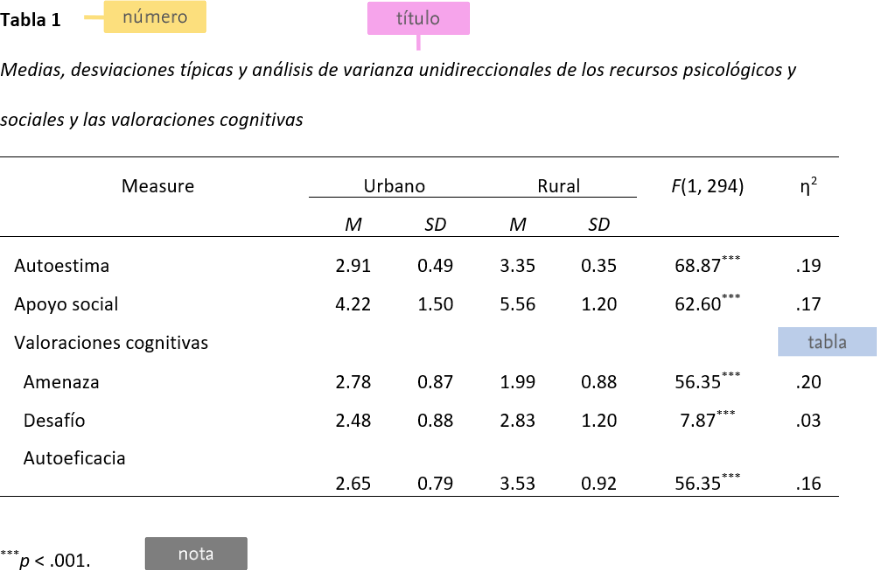
\includegraphics[width=1\linewidth]{images/screenshot022}
			\end{figure}

		\end{column}
	\end{columns}

\end{frame}

\begin{frame}
	\frametitle{Figura tomada de un artículo científico}

	\begin{columns}[c] % The "c" option specifies centered vertical alignment while the "t" option is used for top vertical alignment
		\begin{column}{0.5\textwidth} % Left column width
			\textbf{Repetir fila de títulos de una tabla }

			Si todo el contenido de tu tabla no entra en una sola página, repite la fila de
			títulos en cada página para facilitar la lectura de los datos. Utilizando Word:

			\begin{enumerate}
				\item 	Seleccionar la fila de títulos de la tabla
				\item 	En el menú superior, clic en Disposición
				\item 	Clic en Repetir filas de títulos
			\end{enumerate}
		\end{column}
		\begin{column}{0.5\textwidth} % Right column width
			\begin{figure}
				\centering
				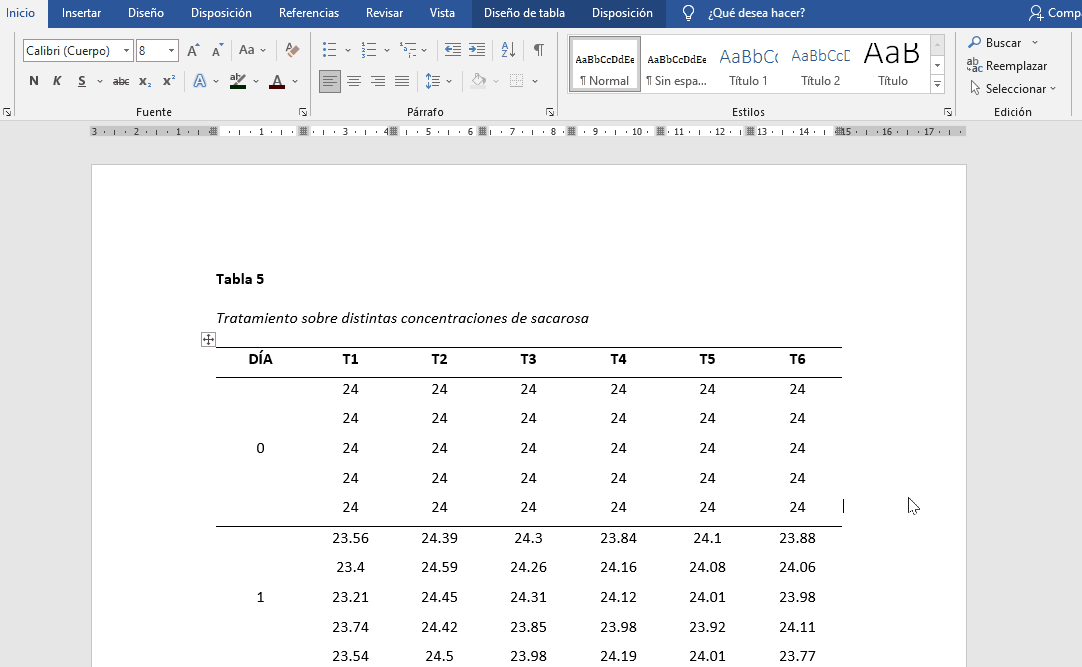
\includegraphics[width=1\linewidth]{images/screenshot023}
			\end{figure}

		\end{column}
	\end{columns}

\end{frame}

\begin{frame}
	\frametitle{Figura tomada de un artículo científico}

	\begin{columns}[c] % The "c" option specifies centered vertical alignment while the "t" option is used for top vertical alignment
		\begin{column}{0.5\textwidth} % Left column width
			\textbf{Correcto}

			\begin{itemize}
				\item 	Como se muestra en la Tabla 3, las características de la población...
				\item 	La Figura 4 muestra el gráfico de dispersión...
				\item 	... como muestran los resultados (ver Tabla 2).
				\item 	ambos modelos (ver Figuras 5 y 8).
			\end{itemize}

		\end{column}
		\begin{column}{0.5\textwidth} % Right column width
			\textbf{Incorrecto}

			\begin{itemize}
				\item 	La siguiente tabla muestra las características de la población...
				\item 	La figura de abajo muestra el gráfico de dispersión...
				\item 	... como muestran los resultados en la tabla superior.
				\item 	como las figuras inferiores permiten ver.
			\end{itemize}

		\end{column}
	\end{columns}

\end{frame}

% Sección 10
\section{Estilos}
\begin{frame}{Estilos}

\end{frame}

% Sección 11
\section{Referencias}
\begin{frame}{Referencias}

\end{frame}

%----------------------------------------------------------------------------------------
%	CLOSING SLIDE
%----------------------------------------------------------------------------------------

\begin{frame}[plain] % The optional argument 'plain' hides the headline and footline
	\begin{center}
		{\Huge The End}

		\bigskip\bigskip % Vertical whitespace

		{\LARGE Questions? Comments?}
	\end{center}
\end{frame}

%----------------------------------------------------------------------------------------
\end{document}
